\chapter{Path Integral Quantum Annealing}

Spin glasses are magnetic systems where individual contributions to the Hamiltonian are conflicting with each other. This is the result of an intrinsic structural disorder present in the system, an example of which can be seen in figure \ref{fig:frustration}. One of the interesting properties of such a system is called freezing. During freezing the disorder increases as a function of some order parameter and the system can get stuck in local minima, becoming trapped in a meta-stable configuration that has higher energy than the ground state  \cite{Binder1986}. Due to the lack of exact solutions for most spin glasses we have to resort to numerical approximations to study the behaviour of such systems. 
\begin{figure}[h]
    \centering
    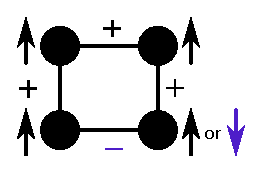
\includegraphics{figures/chapter2/frustration.eps}
    \caption{Toy example of a frustrated system. The bottom right spin can be both in state $+$ or $-$ since both give an equal contribution to the total energy of the system, leading to frustration \cite{Mydosh2015}.}
    \label{fig:frustration}
\end{figure}
We will study the Edwards-Anderson spin glass to get acquainted with some of the computational techniques in quantum many body physics. We reproduce the original results by Santoro \cite{Santoro2002} and we summarize almost the almost 2 decade spanning discussion about the efficiency and and physical interpretation of quantum annealing (QA). Through the use of the Trotter-Suzuki expansion, we perform simulated quantum annealing to find the ground state of a frustrated spin lattice. This problem is solvable in polynomial time for random nearest neighbour interactions and the exact ground state for an $80\times80$ can be obtained from the K\"oln Spin Glass server \cite{spinglass}. All the code was written in Python3 with the Monte Carlo schedule implemented in Cython for performance. 

\section{Combinatorial Optimization}
The interest in finding an efficient solution of the Edwards-Anderson besides its physical properties is the relation to combinatoric optimization problems. In combinatorial optimization problems we are interested in the "optimal" element of some set. Our problem statement defines what the requirement is for this element to be optimal. A well known example is the travelling salesman problem. Consider a graph $G = (V,E)$ where every vertex is connected with each other vertex (complete). The edges carry a weight $w_{ij}$ that can be seen as the distance between the vertices. One can now ask: what is the shortest route through the graph where we pass each vertex exactly once? In other words: what is the shortest Hamiltonian path through the graph? The amount of possible paths scales exponentially and a brute force search through all the permutations would take $\mathcal{O}(n!)$ operations and would already be problematic for about 20 cities. To solve this problem we rely on heuristic methods that give an approximate solution very close to the optimal one. There are a lot more problems that scale exponentially with the system size and for a specific class of problems (NP-Complete), it can be shown mathematically that it is possible to map each problem onto another one in polynomial time \cite{Lucas2014}. This suggests that it might be more efficient to map the problem 1 onto problem 2, if a more efficient algorithm exist for problem 2 and the cost of the mapping is not too high. Finding the ground state of a spin glass is another example of an exponentially hard problem. If we map a combinatorial problem of interest to the spin glass, we can solve this problem by finding the ground state. Consider the Edwards-Anderson model Hamiltonian which is known to have a glassy phase at low temperature:
\begin{equation}
    H_{EA} = -\sum_{\langle ij \rangle} J_{ij} s_i s_j
    \label{ham_EA}
\end{equation}
Here Ising spins $(s_i=\pm 1)$ occupy the sites of a $d$-dimensional cubic lattice, and $J_{ij}$ are the random couplings between nearest-neighbor sites drawn from some prescribed distribution. When the couplings $J_{ij}$ fluctuate randomly without a definite sign, the Hamiltonian \ref{ham_EA} describes a frustrated and disordered system \cite{Nishimori2001}. Finding the ground state is again exponentially hard, but decades of research into spin models has made their statistical properties well understood and a lot of good approximate methods exist for finding the ground state. \newline

One of those methods is Simulated Quantum Annealing (SQA), which uses the adiabatic theorem of quantum mechanics to find the ground state in an efficient manner. To do this, we start with a quantum system in the ground state of another Hamiltonian $H_0$ that can be simply realized in an experimental setup. We then slowly adjust the system so that it is governed by the dynamics of the desired Hamiltonian $H_P$. After the annealing procedure we hope to find the system to be in the ground state of the desired Hamiltonian.
\begin{equation*}
    H(t) = \left(\mathbb{1} - \frac{t}{T} \right) H_0 +  \frac{t}{T} H_P
\end{equation*}
If $T$ is large enough and $\comm{H_0}{H_P}\neq0$ then the system remains in the ground state at all times $t$ for small enough time steps. However, if the distance between the first excited state and ground state becomes exponentially small, then the time $T$ it requires to keep the system in the ground state becomes exponentially large. Quantum annealing is an adiabatic scheme where we introduce a transverse field on each spin site and slowly reduce it to zero. Building a computational device that performs quantum annealing is an intense field of research and which we will discuss briefly in section \ref{sec:qa_debate}. We can also simulate quantum annealing efficiently for relatively large systems ($80\times80$ spins) by using a path integral Monte Carlo approach. Before introducing this we will briefly review its classical counterpart, simulated annealing.

\section{Simulated Annealing}

First let us repeat some basic statistical mechanics knowledge that we will require for solving this problem. At finite temperature, we have to use a statistical ensemble of states to determine the expectation value of a physical observable of interest.
\begin{align*}
\langle A \rangle &= \sum_i P_i A_i\\
 P_i &= \frac{e^{-\beta E_i}}{\sum_j e^{-\beta E_j}} =  \frac{e^{-\beta E_i}}{Z}& 
\end{align*}
with inverse temperature $k_b\beta=\frac{1}{T}$ (we set $k_b=1$ from now). The distribution for $P_i$ is known as the Boltzmann distribution with $Z$ the grand canonical partition function. For determining the value of an observable, or finding the ground state (the most likely state of the system), we need to determine $P_i$. However, for a system with $N$ spins that has $2$ degrees of freedom this means we have $2^N$ possible configurations, so our number of states scales exponentially with the number of spins we add. This means that estimating $P_i$ becomes more complicated if the system increases with size, since we have to sum all possible states of the system, so the partition sum $Z$ becomes large. A solution to this problem is using a Markov Chain Monte Carlo sampling algorithm to find the most relevant contributions to the partition function. The partition function is our stationary distribution over possible configurations of the system. Markov chains approximate this stationary distribution of our system, because they tend to move towards likely configurations of the system that dominate the contribution to the partition function. Markov Chains have to satisfy detailed balance, which means that
\begin{align*}
    P_i W_{i\rightarrow j} = P_j W_{j\rightarrow i}
\end{align*}
With $W_{i\rightarrow j}$ the transition matrix between state $i$ and $j$. The system also has to be ergodic, which means that all states in the system are accessible. This condition is satisfied if 
\begin{align*}
    W_{i\rightarrow j} >0
\end{align*}
An example of an algorithm which has this property is the Metropolis-Hastings algorithm. We take $P_i = \frac{e^{-\beta E_i}}{Z}$, which allows us to divide out the partition sum, and only look at the difference between the energies $\Delta E = E_i - E_j$.
\begin{align*}
    e^{-\beta \Delta E} W_{i\rightarrow j} = W_{j\rightarrow i}
\end{align*}
If we take 
\begin{equation*}
    W_{j\rightarrow i} = \min\{1, e^{-\beta \Delta E} \}
\end{equation*}
then it is clear that detailed balance is satisfied. To obtain samples of our distribution we start in a random state of our system and attempt spin flips based on the transition probability $W_{i\rightarrow j}$. We have to compare with a uniform number $r \sim \mathcal{U}(0,1)$, to ensure that we transition to the desired state with proposed transition probability $W_{i\rightarrow j}$. By generating chains of sufficient length we can approach the target distribution $P_i$ with an empirical distribution of sampled states. With these sampled states we can obtain a reasonable approximation for the expectation values of desired observables.\newline
If we perform this Monte Carlo schedule at a certain temperature $\beta$, it is possible that thermal fluctuations are too strong to give us the interesting states of the system. If the temperature is too low, it is possible that we get stuck in local minima and are unable to properly explore the full state space. To resolve these problems one can perform simulated annealing (SA), where the system is cooled from an initial temperature $\beta_0$. This heuristic is relatively efficient for solving combinatorial optimization problems, such as the traveling salesman problem. It has been shown that if the cooling schedule is sufficiently slow, so $\beta(k) \geq \frac{\log(1+k)}{c}$ where $k$ is the $k$-th site replacement and $c$ some constant, then we will always find the global minimum of the cost function \cite{Geman1984}. A schematic representation of this behaviour is given in figure \ref{fig:sa}.
\begin{figure}[htb!]
    \centering
    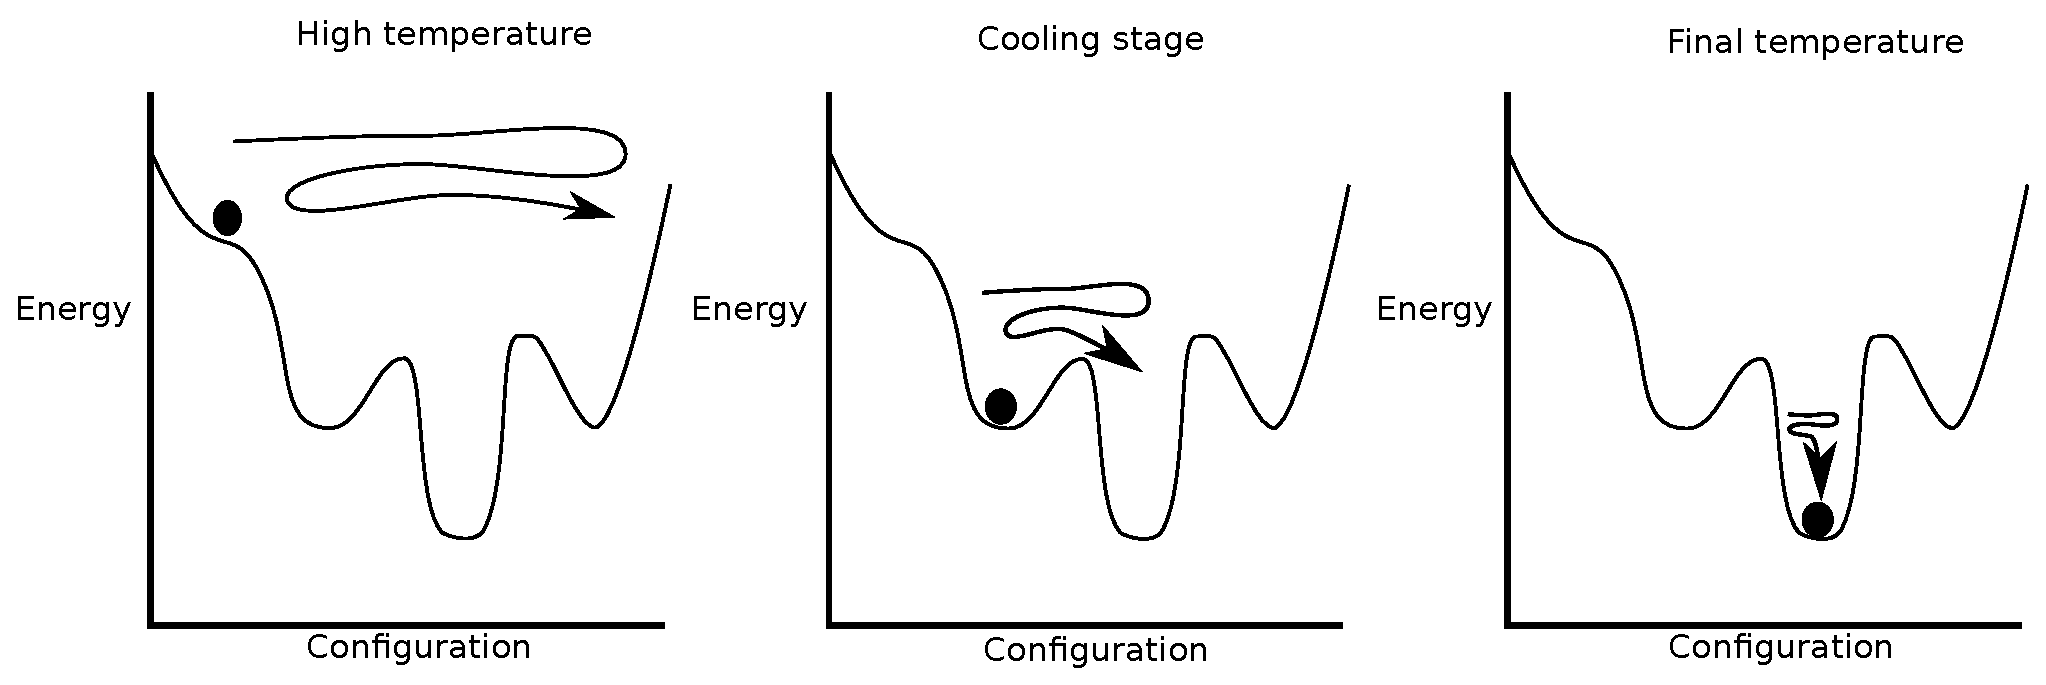
\includegraphics[width=\textwidth]{figures/chapter2/SA.eps}
    \caption{Schematic representation of SA. Thermal fluctuations at high temperature allow for a more thorough exploration of the state space. When cooling we slowly limit these fluctuations and hope to reach the global minimum when the dynamics freeze.}
    \label{fig:sa}
\end{figure}

\section{Simulated Quantum Annealing}

The underlying principle of SA is that thermal fluctuations allow random jumps over energy barriers to take place while searching for the global minimum. The height of this barrier affects the probability of hopping over it. But we are not limited to thermal fluctuations. By adding a transverse field $\Gamma$ that is orthogonal to the spin orientation, we can allow for quantum fluctuations that ensure that tunneling between states becomes possible, so that we can tunnel through an energy barrier. This method gives us another meta-heuristic for finding the ground state of a spin glass. By mapping a two-dimensional Ising model onto a two-dimensional+1 system of interacting classical spins lattices, we can efficiently simulate quantum annealing.
\begin{figure}[htb!]
    \centering
    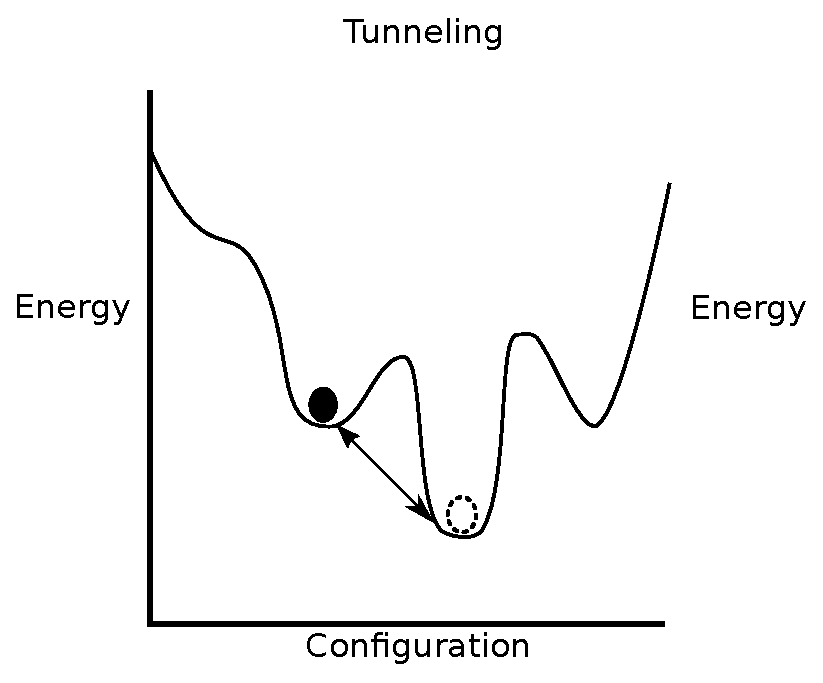
\includegraphics[width=0.5\textwidth]{figures/chapter2/QA.eps}
    \caption{Schematic representation of SQA. The random probability of moving to another configuration is now affected by the width of the barrier, instead of the height.}
    \label{fig:qa}
\end{figure}
First, we rewrite our Hamiltonian in terms of the Pauli spin matrices $\sigma_i$:
\begin{equation}
    H = -\sum_{\langle ij \rangle} J_{ij} \sigma^z_i \sigma^z_j - \Gamma \sum_i \sigma^x_i
    \label{ham_EA_q}
\end{equation}
so each Pauli operator works on a specific spin site $i$, where the Pauli operators are defined as in equation \ref{eq:pauli_mats}. The Hamiltonian is now described as an operator in the product Hilbert space of all the individual spin sites.
\begin{align*}
    \mathcal{H} = \bigotimes_i^N \mathcal{H}_i
\end{align*}
with $\text{dim}(\mathcal{H})= \prod_i^N \text{dim}(\mathcal{H}_i) = 2^N$.
We can separate our Hamiltonian in a classical and quantum mechanical part $H = H_{cl}+H_{qm}$
\begin{eqnarray}
    H_{cl} &=& \sum_{\langle ij \rangle} J_{ij} \sigma_i^z\sigma_j^z \text{ where } \sigma_j^z = \left( \bigotimes_{k=1}^{i-1}\mathbb{1} \right)\otimes\sigma^z\otimes\left(\bigotimes_{l=i+1}^{N}\mathbb{1}_K\right)\nonumber\\
    H_{qm}&=&\sum_{i=1} \sigma_j^x \text{ where }\sigma_j^x = \left( \bigotimes_{k=1}^{i-1}\mathbb{1} \right)\otimes\sigma^x\otimes\left(\bigotimes_{l=i+1}^{N}\mathbb{1}\right)\nonumber
\end{eqnarray}
Here $\mathbb{1}$ is a $2\times2$ identity matrix and $\otimes$ is the Kronecker-product. We can construct a density matrix at temperature $T$ from this Hamiltonian.
\begin{equation*}
    \rho = \frac{e^{-\beta H }}{\Tr{e^{-\beta H }}}
\end{equation*}
The calculation of the expectation value of an operator at finite temperature is given in definition \ref{def:density_mat} and gives
\begin{equation}
    \langle \hat{A} \rangle = \Tr{\hat{A}\rho}=\frac{\Tr{\hat{A} e^{-\beta H }}}{\Tr{e^{-\beta H }}}
\end{equation}
Note that if we have our classical model, without transverse field, then the Hamiltonian becomes diagonal in the $\sigma^z$ basis, so the traces simply reduce to a sum and we get back our standard Boltzmann distribution. As before, for a small system we can perform the traces for a system because we can construct the Hamiltonian explicitly through the tensor product. However, the full Hamiltonian has to be represented by a $2^N\times2^N$ matrix, which already becomes problematic for around 20 spins. However, we can greatly simplify the calculations. First we write out the exponential
\begin{equation*}
    e^{-\beta H} = e^{-\beta (H_{cl}+H_{qm})}
\end{equation*}
Unfortunately it is only possible to write $e^{A+B} = e^A e^B$ if the matrices $A$ and $B$ commute, which is not the case for our two Hamiltonians. However with the Trotter formula we can write
\begin{equation*}
    e^{A+B} = \lim_{M\rightarrow\infty} \left( e^{A/M}e^{B/M} \right)^M
\end{equation*}  
so that for finite $M$ we can write
\begin{equation*}
e^{-\beta/M H} \approx \left(e^{-\beta/M H_{cl}}e^{-\beta/M H_{qm}}\right)^M
\end{equation*}
at the cost of an error of order $\mathcal{O}\left((\frac{\beta}{M})^2\right)$, proportional to the Trotter breakup time $M$. This allows us to write the partition function as
\begin{equation*}
Z \approx \Tr{\left(e^{-\beta/M H_{cl}}e^{-\beta/M H_{qm}}\right)^M}
\end{equation*}
Using the completeness relation $\sum_{s^i} \ket{s^i}\bra{s^i} = 1_{2^N}$, where $\ket{s^i} \in \{|s^1\rangle,...,|s^{2^N}\rangle\}$ is an orthonormal basis of our system. This basis can be written as a tensorproduct of eigenvectors of individual spin site.
\begin{equation*}
    \ket{s^i} = \bigotimes_k^N \ket{s^i_k} = \overbrace{
    \begin{pmatrix}
    1 \\
    0
    \end{pmatrix}
    \otimes
    \begin{pmatrix}
    0 \\
    1
    \end{pmatrix}
    \otimes\ldots \otimes
    \begin{pmatrix}
    1 \\
    0
    \end{pmatrix}}^{N \text{ times}}
\end{equation*}
We write the trace as
\begin{align*}
\Tr{\left(e^{-\beta/M H_{cl}}e^{-\beta/M H_{qm}}\right)^M}  &= \Tr\bigg\{\overbrace{\left(e^{-\beta/M H_{cl}}e^{-\beta/M H_{qm}}\right) \times 1_{2^N}  \times ... \times 1_{2^N} \times \left(e^{-\beta/M H_{cl}}e^{-\beta/M H_{qm}}\right) }^{\text{$M$ times}}\bigg\}\\
 &=\Tr\bigg\{\sum_{s^1}...\sum_{s^M} \left(e^{-\beta/M H_{cl}}e^{-\beta/M H_{qm}}\right)  \times \ket{s^1}\bra{s^1}  \times...\\
 & \ldots \times\ket{s^M}\bra{s^M} \times  \left(e^{-\beta/M H_{cl}}e^{-\beta/M H_{qm}}\right) \bigg\}\\
 &=\sum_{s^1}...\sum_{s^M} \bra{s^1}\left(e^{-\beta/M H_{cl}}e^{-\beta/M H_{qm}}\right) \times \ket{s^2}\bra{s^2}  \times... \\ 
 & \ldots\times\ket{s^M}\bra{s^M} \times  \left(e^{-\beta/M H_{cl}}e^{-\beta/M H_{qm}}\right)\ket{s^1}\\
\end{align*}
Note that we assume periodic boundary conditions so that $\ket{s^{M+1}}=\ket{s^1}$. The classical part of the Hamiltonian is diagonal in the chosen spin basis
\begin{equation*}
    H_{cl} = \sum_{\langle ij \rangle} J_{ij} \sigma^z_i \sigma^z_j
\end{equation*}
where we remember that the eigenvalues of the $\sigma^z$ matrices are $+1$ and $-1$.
\begin{equation*}
    \sigma^z_j \ket{s^k} = \pm  \ket{s^k}
\end{equation*}
This gives for the term in the Hamiltonian
\begin{equation*}
      \bra{s^k}\sigma^z_i \sigma^z_j  \ket{s^{k+1}} = \begin{cases}
      +1 \text{ if spins at site $i$ and $j$ are aligned parallel}\\
      -1 \text{ if spins at site $i$ and $j$ are aligned anti-parallel}
      \end{cases}
\end{equation*}
We can pull this term out of the state sandwich, since =$H_{cl}^k$ is diagonal in the basis $\{\ket{s^k}\}$
\begin{equation*}
    \bra{s^k} \exp\left(-\frac{\beta}{M}H_{cl}^k\right) \exp\left(-\frac{\beta}{M} H_{qm}\right) \ket{s^{k+1}} = \bra{s^k} \exp\left(-\frac{\beta}{M} H_{qm}\right) \ket{s^{k+1}} \exp\left(-\frac{\beta}{M}H_{cl}^k\right)
\end{equation*}
where 
\begin{eqnarray*}
    \exp\left(-\frac{\beta}{M} H_{cl}^k\right) = \exp\left(\frac{\beta}{M}\sum_{\langle ij \rangle} J_{ij} s_i^k s_j^k \right) 
\end{eqnarray*}
The vectors $s_i^k$ are simply classical spin vectors with $+1$ and $-1$ for the respective up and down states. So the classical energy contribution to our partition function is equal in each of the $M$ copies of the spin system. The only non-trivial term is the sandwich $\bra{s_k} \exp\left(-\beta/M H_{qm}\right) \ket{s_{k+1}}$, which is dependent on the coupling between copies $k$ and $k+1$.
\begin{eqnarray*}
    \bra{s^k} \exp\left(-\frac{\beta}{M} H_{qm}\right) \ket{s^{k+1}} &=& \bra{s^k} \exp\left(\frac{\beta\Gamma}{M} \sum_i \sigma_i^x\right) \ket{s^{k+1}}\\
    % &=& \prod_i^N \bra{s^k_i} \exp\left({\frac{\beta\Gamma}{M}\sigma_i^x}\right) \ket{s^{k+1}_i}\\
\end{eqnarray*}
So the Pauli operator only works the individual spins $\ket{s^k_i}$. We can use the identity \cite{Das2014}
\begin{equation*}
    e^{a \sigma^x} = e^{-i (i a \sigma^x)} = \cos(i a \sigma^x) - i \sin(i a \sigma^x) = \cosh{a} + \sigma^x \sinh{a}
\end{equation*}
where $\sigma_x$ works as a flip operator
\begin{align*}
    \sigma^x \ket{\uparrow} = \ket{\downarrow} \text{ and }
    \sigma^x \ket{\downarrow} = \ket{\uparrow}
\end{align*}
It is then easy to see that
\begin{align*}
    &\bra{\uparrow} e^{a\sigma^x} \ket{\uparrow} = \bra{\downarrow} \exp\left({a\sigma^x}\right) \ket{\downarrow} = \cosh{a} \\
    &\bra{\uparrow} e^{a\sigma^x} \ket{\downarrow} = \bra{\downarrow} \exp\left({a\sigma^x}\right) \ket{\uparrow} = \sinh{a}
\end{align*}
where we note that
\begin{align*}
    &\cosh{a} = \left(\frac{1}{2} \sinh{2a} \cdot \coth{a}\right)^{\frac{1}{2}}\\
    &\sinh{a} =  \left(\frac{1}{2} \sinh{2a} / \coth{a}\right)^{\frac{1}{2}}
\end{align*}
This means that we have two separate cases, if the spins are of equal sign, we pick up a $\left(\coth{a}\right)^{\frac{1}{2}}$ and otherwise a $\left(\coth{a}\right)^{-\frac{1}{2}}$ term. To account for this we write
\begin{eqnarray*}
    \bra{s^k_i} \exp\left(\sum_i \frac{\beta\Gamma}{M}\sigma_i^x\right) \ket{s^{k+1}_i} = \overbrace{\left(\frac{1}{2} \sinh{\frac{2\beta\Gamma}{M}}\right)^{\frac{N}{2}}}^{\text{spin independent}} \overbrace{\exp\left(\sum_i \frac{1}{2}\ln{\left(\coth{\frac{\beta\Gamma}{M}}\right)}s_i^k s_i^{k+1}\right)}^{\text{spin dependent}}
\end{eqnarray*}
Putting everything together we get 
\begin{align}
    Z &\approx \prod_{k=1}^M \sum_{s^k} \left(\frac{1}{2} \sinh{\frac{2\beta\Gamma}{M}}\right)^{\frac{N}{2}} \exp\left(\frac{\beta}{M}\sum_{\langle ij \rangle} J_{ij} s_i^k s_j^k - \sum_i\frac{1}{2}\ln{\left(\tanh{\frac{\beta\Gamma}{M}}\right)}s_i^k s_i^{k+1}\right)\nonumber\\
    &= \prod_{k=1}^M \sum_{s^k}C^{\frac{N}{2}} \exp\left(\frac{1}{MT}\left[\sum_{\langle ij \rangle} J_{ij} s_i^k s_j^k - \sum_i\frac{MT}{2}\ln{\left(\tanh\frac{\beta\Gamma}{M}\right)}s_i^k s_i^{k+1}\right]\right)\label{eq:trotter_part}
\end{align}
So we have a product over all Trotter-slices, a sum over all possible configurations per slice, a sum over nearest neighbour spins and sum over spins connected through the duplicate slices. Conceptually this means is that in order to approximate our quantum mechanical partition sum, we create $M$ copies of our system with classical energy $H_{cl}$ and an interaction between the copies. \newline 
This can be seen as a Feynman-Kac path integral, where we perform variation w.r.t. the imaginary time $i\tau = \frac{\beta}{M}$. So we have mapped the static two-dimensional quantum system to a classical system of dimension $2+1$, evolving in imaginary time. 
\begin{figure}
    \centering
    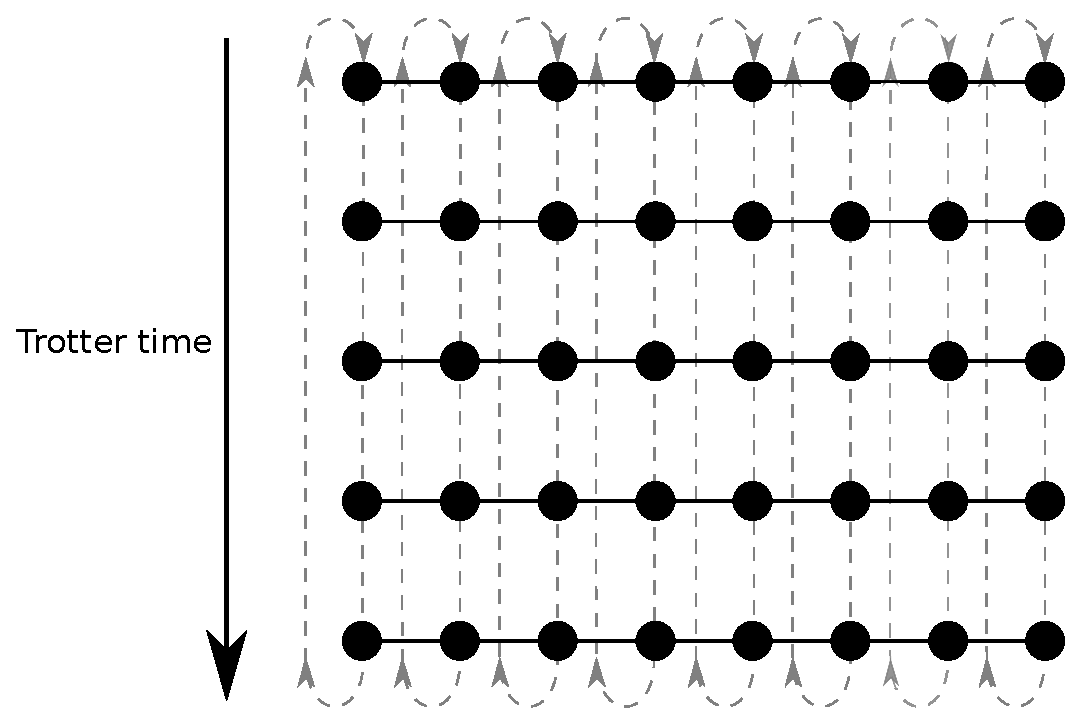
\includegraphics[width = 0.5\textwidth]{figures/chapter2/trotter.eps}
    \caption{Schematic representation of imaginary time slices representing the quantum system. Each horizontal line represent a copy of the two-dimensional lattice. These copies are connected by an interaction that is dependent on $\beta$, $\Gamma$ and $M$. Due to its relation to the path integral, the vertical direction is called the Trotter time.}
    \label{fig:trotter}
\end{figure}
A measure of Monte Carlo time that is often used is the Monte Carlo step per site (MCS/site or $\tau$) which corresponds to the attempted flip of every spin in the system once \cite{landau2014}. \newline

With this imaginary time slice description, we can apply the Metropolis-Hastings Monte Carlo algorithm to perform variation with respect to each time slice and again approximate the distribution of states $P_i$. We can obtain a rather simple description of the difference in energies with the help of equation \ref{eq:trotter_part}. A spin flip at site $s^k_i$ for some configuration $\{s^k\}$ results in a difference in energy of 
\begin{align*}
    \Delta E_{loc} \propto -2 \sum_{\langle ij \rangle}^N J_{ij} s_i^k s_j^k + MT\ln{\left(\tanh{\frac{\Gamma}{MT}}\right)}\left[s_i^{k-1} s_i^{k} + s_i^k s_i^{k+1}\right]
\end{align*}
This is considered a local move, which we apply to all sites in all slices. In other words, we vary the path integral in space, while keeping the time constant. We can also perform a global move, which means flipping a spin at location $i$ in every slice $k$. Clearly this has no impact on the field dependent term, because this contains only terms quadratic in the flipped spin. 
\begin{align*}
    \Delta E_{glob} \propto -2 \sum_{k=0}^M\sum_{\langle ij \rangle}^N J_{ij} s_i^k s_j^k
\end{align*}
The full algorithm consists of first performing a single local move on all sites in the $k$-th lattice and then performing a global move for all sites. This is done for each field $\Gamma(t)$ in our annealing schedule. This annealing schedule consists of linearly decreasing the field from some initial value $\Gamma_i=3$ to a final value close to zero $\Gamma_f=10^{-9}$, so that we retrieve the original classical Hamiltonian. This annealing schedule consist of $\tau$ steps, where at each step we perform one Monte Carlo step per spin (MCS). The choice of $\Gamma_i$ not trivial. If $\Gamma_i$ is too large, then $\log(\tanh(\Gamma / MT))\approx 0$, which means that the flips are not impacted by slice correlations. For too small $\Gamma_i$, the slice correlations dominate the Monte Carlo dynamics, so the important correlations are drowned by the all the unimportant ones. The temperature is kept constant throughout the procedure, but before we start, we pre-anneal to a single slice to a  fully thermalized state from temperature $\beta_i = 1/3$ to temperature $\beta_f = 1/MT$ and copy this state for all the other slices. 
This choice of thermalizing to a temperature based on the number of Trotter slices is motivated by the face that we want the dynamics to be ergodic so that we can reach all states in our state space. The full system behaves like a collection of noninteracting two-dimensional systems at temperature $MT$. This temperature must be larger than the glass temperature, so that all states can be reached. Since our interactions are of magnitude $|J_{ij}| \approx 1$, we can require that $PT\geq 1$ to ensure that we are not at the glass transition temperature \cite{Santoro2002}. The results of the annealing schedule can be seen in figure \ref{fig:santoro}.
\clearpage
\begin{figure}[htb!]
    \centering
    \makebox[\textwidth][c]{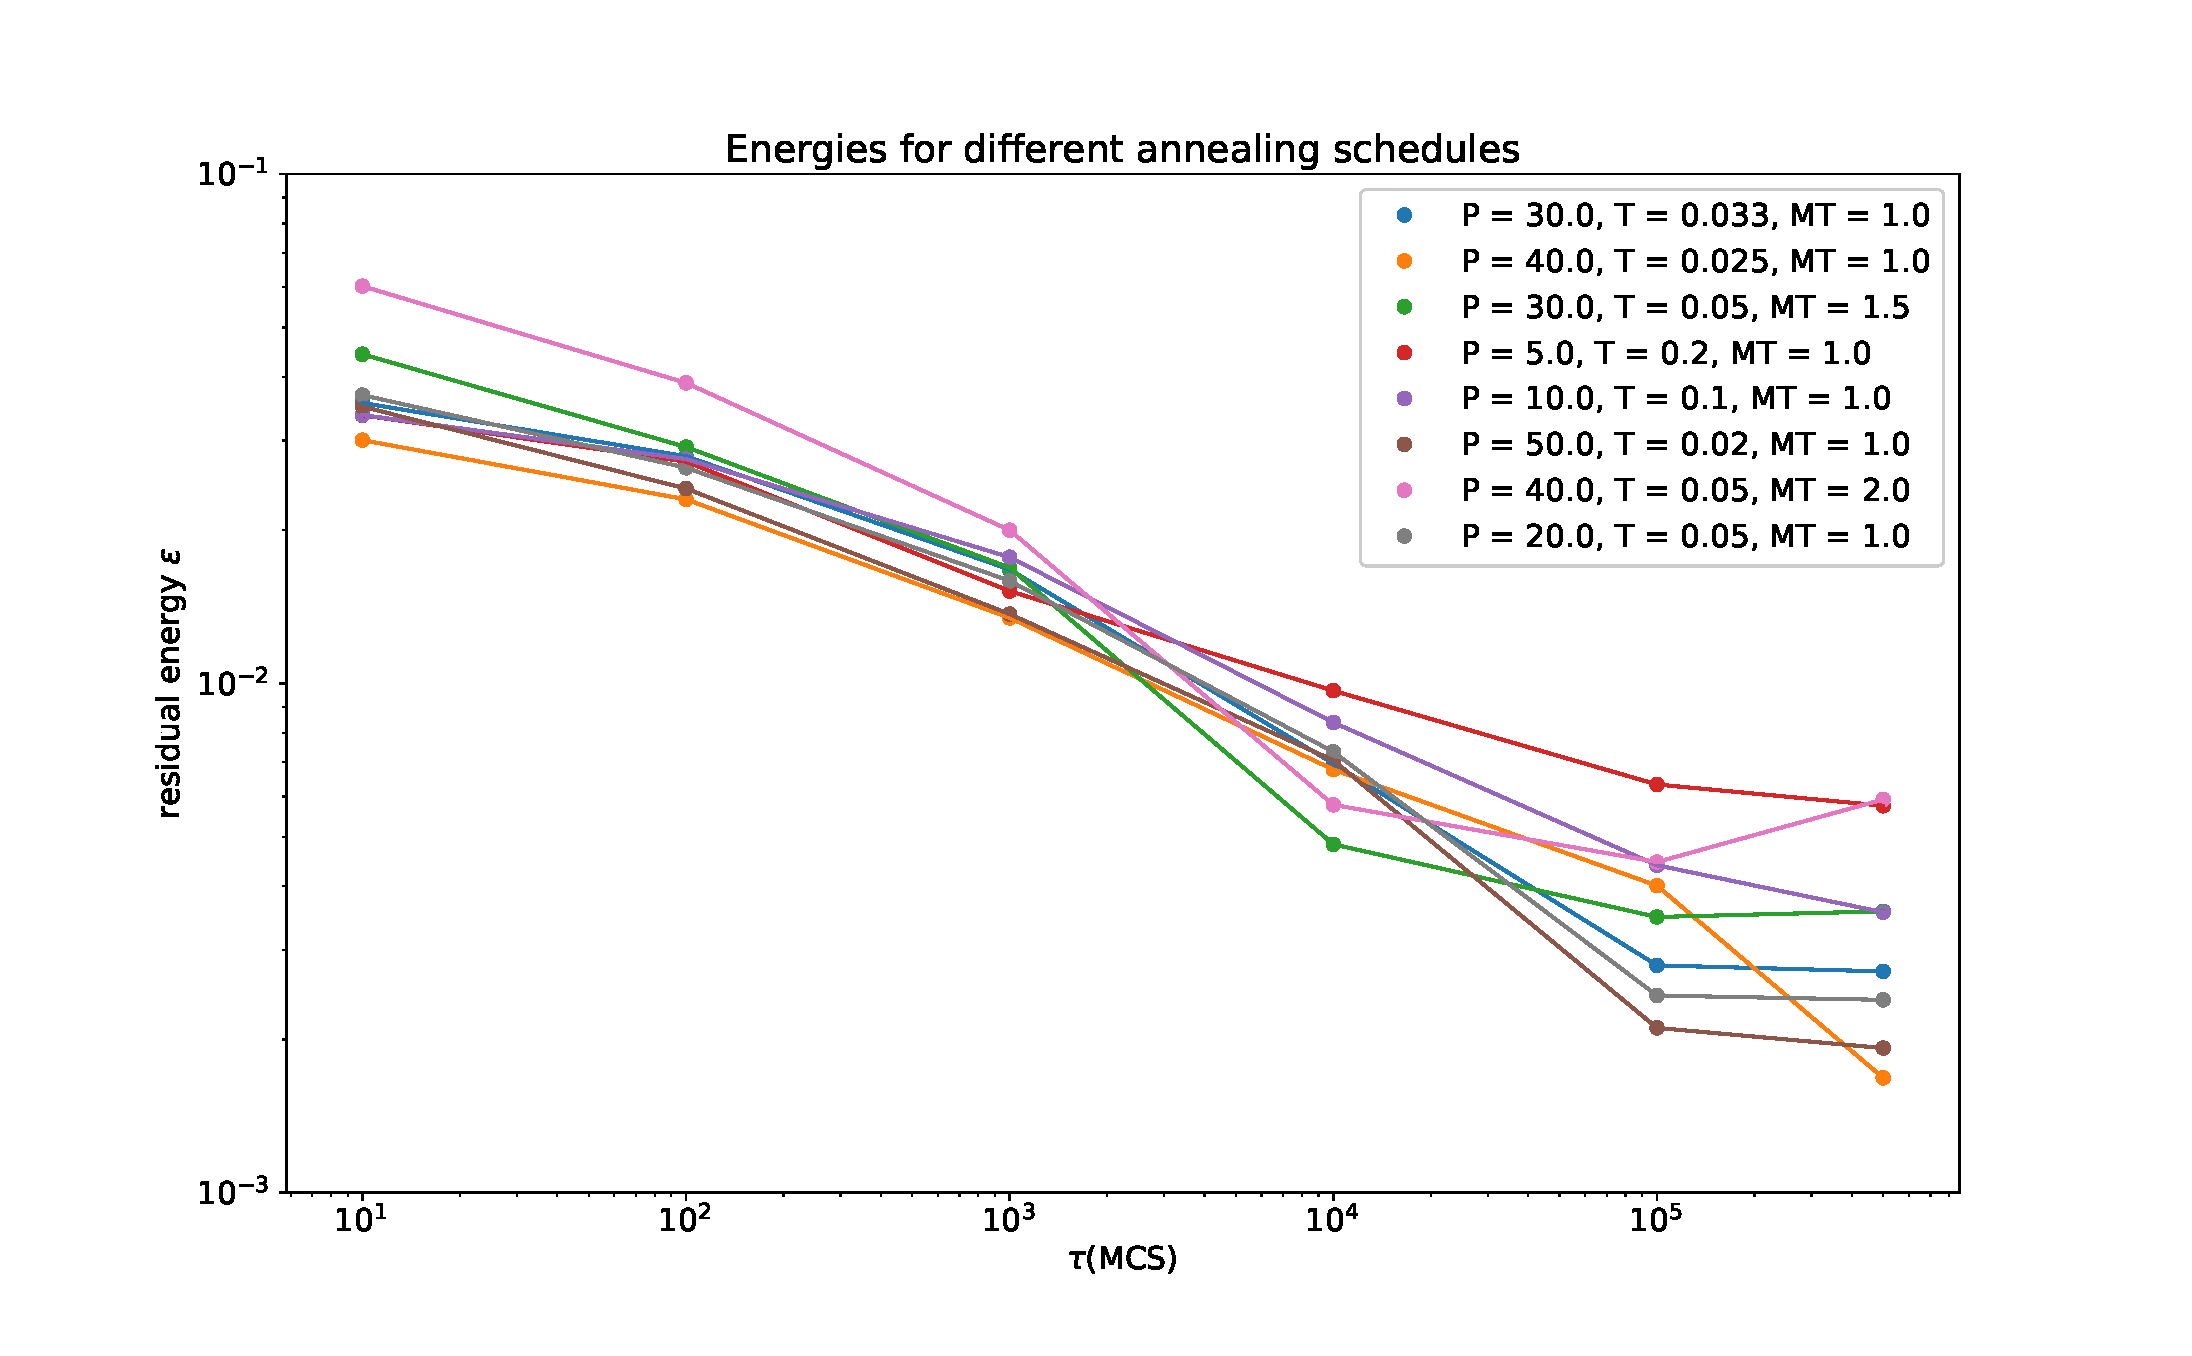
\includegraphics[width=1.2\textwidth]{figures/chapter2/santoro_e_res.eps}}
    \caption{The residual energy $\epsilon = \frac{\abs{E_{QMC} - E_{0}}}{N}$ versus $\tau$, the number of steps in the annealing schedule in terms of MCS. As the field $\Gamma$ slowly reaches zero, the Trotter slices will be slowly forced into the same configuration, as the coupling term between the slices starts to dominate the difference in energy. This means that the effective temperature of our system changes from $MT \rightarrow T$. Santoro \cite{Santoro2002} defines two regimes of the algorithm: a classical freezing regime, where, and quantum freezing regime. \textbf{Classical freezing:} All Trotter slices reach the same configuration in the annealing schedule. This is because the ratio $\frac{\Gamma}{MT}$ becomes small when $\Gamma$ goes to zero, causing the interactions between the slices to dominate the energy differences, forcing all slices into the same configuration. This means that quantum fluctuations can no longer allow for tunneling, and we are simply performing $M$ Monte Carlo schedules in all the non-interacting slices. \textbf{Quantum freezing:} The cause of this classical freezing is that the number of slices $M$ is too small for the resulting couplings (which scale with $MT$) and the schedule of $\tau$ steps. This results in a fast decrease in the number of flips per MCS and a worse final energy found. This figure closely matches Santoro's original results.}
    \label{fig:santoro}
\end{figure}

\section{The Quantum Annealing Debate\label{sec:qa_debate}}

Even though the initial idea was published in 1998 \cite{kadowaki1998}, the dust has still not settled on whether SQA is more efficient than its classical counterpart \cite{Mbeng2018}. 
One of the problems is that the Monte Carlo dynamics (global or local spin flips) of SQA are unrelated to the dynamics of a physical system whose dynamics are governed by the Schr\"odinger equation. Another problem is that when we discretize the path integral into $M$ steps, we should be taking the limit $M\rightarrow\infty$. But if we consider SQA as an optimization algorithm, then one might be interested in finding the optimal $M$ and simply take the lowest energy state out of all the slices. Again there are conflicting results concerning this issue. In \cite{Heim2015} it is reported that if one takes the physical limit of $M\rightarrow\infty$ and measures the average energy over all Trotter slices, the advantage vanishes. The improved scaling is ascribed to the discretiziation of the path integral. On the other hand, replica theory calculations done by \cite{Baldassi2018} show that in the limit $M\rightarrow\infty$ SQA is definitely more efficient than SA. A physical device, built by D-Wave, that is supposed to perform adiabtatic quantum annealing has also sparked a lot of discussion. Some authors report that the device uses quantum effects and provides a noticeable speedup \cite{Boixo2014, Muthukrishnan2016}, while others show that a classical device could have the same operational signature and that a speedup is not really achieved \cite{Smolin2013, Ronnow2014}. More recently it has been shown that one can simulate topological phenomena with this device, giving it use beyond the idea of quantum supremacy \cite{King2018}. The whole discussion is complicated even further because one can not directly compare the device to the simulation because the physicality of the simulation is not undisputed. It is clear that the last word has not been spoken on this topic, further developments of both theory and hardware are necessary to provide more conclusive answers on these issues.

\section{Conclusion}

The original results of simulated quantum annealing have been reproduced. The incorporation of quantum physics into computational methods can be a fruitful method to develop novel algorithms. This is will be the main focus of the next chapter, where we will apply quantum physics to develop a new kind of perceptron algorithm.